\documentclass[9pt,twocolumn,twoside]{../../styles/osajnl}
\usepackage{fancyvrb}
\journal{i524} 

\title{Analysis of USGS Earthquake Data}

\author[1,*]{Nandita Sathe}

\affil[1]{School of Informatics and Computing, Bloomington, IN 47408, U.S.A.}

\affil[*]{Corresponding authors: nsathe@iu.edu}

\dates{project-001, \today}

\ociscodes{I524, geospatial, MongoDB, Plotly, K-means clustering, DBSCAN, Python, pymongo, USGS, Ansible, Cherrypy}

\doi{\url{https://github.com/cloudmesh/sp17-i524/blob/master/project/S17-IO-3017/report/report.pdf}}



\begin{abstract}
Big Data Analytics tools allow us to analyze the huge volumes of geo-spatial data. Data of earthquakes that take place globally is a major part of crucial geo-spatial data. US Geological Survey's (USGS) Earthquake Hazards Program monitor and report earthquakes, assess earthquake impacts and hazards, and research the causes and effects of earthquakes \cite{www-usgs1}. Machine learning algorithms are used for advanced data analysis and earthquakes prediction.
\newline
\end{abstract}

\setboolean{displaycopyright}{true}

\begin{document}

\maketitle

\section{Introduction}

USGS collects volumes of geospatial data pertaining to earthquakes and makes it available for analysis. The project obtains a chunk of the data using GeoJSON web service provided by USGS. The data is saved locally in MongoDB database. Data is analysed using machine learning algorithms. The output is plotted (rendered) on web browser. A light weight web server is used to respond to the web requests. Project is capable of running in cloud environment. Deployment is automated using Ansible. 

\section{Technologies Used}

Technologies used for development and deployment of this project are listed below.
\begin{enumerate}

\item Cloudmesh - For connecting to different cloud environments.
\item Ansible -For deploying software and associated packages.
\item Python - Writing script for data analysis and data processing 
\item Mongo-DB - For storing Geo-spatial data
\item Plotly - As a visualization tool
\item Scikit-learn - For classification of data into clusters 
\item Cherrypy - For web server development 
\end{enumerate}

\section{Background}

\subsection{USGS Web Service and Data Set}
USGS earthquake data is fetched using the web service and passing relevant parameters to it. Out of the voluminous world-wide data of decades this project uses data of earthquakes appeared in North and South America for duration of 2 years from 2015-1-1 till 2017-1-1, having magnitude over 4. To select North and South America region data, its Latitude and Longitude are taken from Search Earth Catalog tool provided by USGS. \cite{www-usgs3}. Web service returns data in JSON format.

\subsection{Data Processing and Visualization}

{\bfseries Severity of earthquakes.} Severity of earthquakes is analysed by their magnitude and depth. Data is classified into clusters using K-Means clustering algorithm (Section 4.1). Clusters are plotted on a interactive scatter plot.

{\bfseries Region affected the most by earthquakes}. Analysing Latitude (lat)-Longitude (lon) of epicenter of the earthquake shows the regions where earthquakes are frequent. Lat lon data is clustered using DBSCAN algorithm (Section 4.2). Clusters are plotted on a geo-scatter plot on a world map.

\section{Implementation}

\subsection{K-Means Clustering}
Given a target number, \emph k, of clusters to find, K-means algorithm locates the centers of each of those \emph k clusters and the boundaries between them. It does this using the following algorithm \cite{www-kmeans}.
\begin{itemize}
    
    \item Step 1: Start with a randomly selected set of \emph k centroids 

    \item Step 2: Determine which observation is in which cluster, based on which centroid it is closest to (using the squared Euclidean distance. 
    \[   \sum_{j=1}^p (x_{ij} - X_{i^1j})^2   \]
    
    where \emph p is the number of dimensions)
    
    \item Re-calculate the centroids of each cluster by minimizing the squared Euclidean distance to each observation in the cluster
    
    \item Repeat 2. and 3. until the members of the clusters (and hence the positions of the centroids) no longer change.

\end{itemize}

\subsection{DBSCAN}
DBSCAN (Density-Based Spatial Clustering of Application with Noise) is a clustering algorithm. Given a set of points in some space, it groups together points that are closely packed together (points with many nearby neighbors), and marks points as outliers if they lie alone in low-density regions. Unlike K-Means Clustering, DBSCAN doesn't need to specify the number of clusters as it finds all the clusters that satisfy the requirement. Following points summarize the algorithm \cite{www-dbscan}.

\begin{itemize}
    \item Step 1: For each point in the data set, an n-dimensional sphere of radius \emph epsilon is drawn around the point (if you have n-dimensional data).
    
    \item Step 2: If the number of points inside the sphere is larger than \emph min-samples, the center of the sphere is set as a cluster, and all the points within the sphere belong to this cluster.
    
    \item Step 3: Loop through all the points within the sphere with the above 2 steps, and expand the cluster whenever it satisfy the 2 rules.
    
    \item Step 4: For the points, which do not belong to any cluster, are treated as outliers. 
\end{itemize}

\subsection{Ansible}

Project is deployed using ansible. Ansible is an automation platform, that automates cloud provisioning, configuration management, application deployments, etc. Ansible jobs are collected in a playbook and run on virtual clusters provided by Chameleon cloud. The tasks include cloning the git repository, installing dependencies and installing MongoDB.

\subsection{Application}
Application has a Cherrypy web server and python scripts that use the web server to send the output in the form of response so that users can see the output of the application in web browser.

Figure \ref{fig:figure1} shows default page showing application usage.

\begin{figure}[htbp]
\centering
\fbox{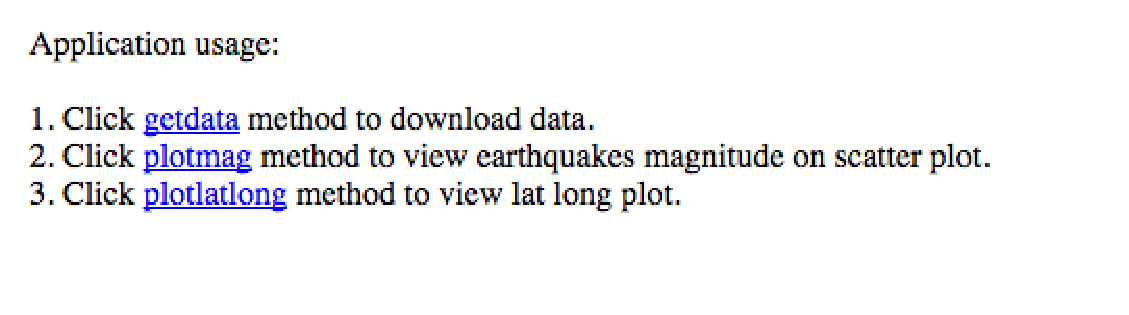
\includegraphics[width=\linewidth]{images/figure1}}
\caption{Application usage} 
\label{fig:figure1}
\end{figure}

\subsection{Steps to Execute}

Steps to execute the project are explained in detail in README.md file \cite{readme-001}.

\section{Execution Plan}

This is how the project is executed on week-by-week basis. 

\begin{enumerate}

\item {\bfseries 13 Mar 2017 - 19 Mar 2017} Research on USGS data and fetching it. Deploy Mongo DB and Mongo Express tool to fetch data from Mongo DB. Data analysis and finalizing the analysis for project.

\item {\bfseries 20 Mar 2017 - 26 Mar 2017} Write script in Python for downloading USGS data at run-time and storing in local MongoDB. Research on clustering algorithms. 

\item {\bfseries 27 Mar 2017 - 02 Apr 2017} Implement K-Means clustering and DBSCAN clustering in sample project. Understand the result. Create a VM on Chameleon. 

\item {\bfseries 03 Apr 2017 - 09 Apr 2017} Write Python script to read data from MongoDB, implement K-Means clustering algorithm. Research on Plotly. Plot clustering result using Plotly. 

\item {\bfseries 10 Apr 2017 - 16 Apr 2017} Implement DBSCAN clustering and plot clustering result using Plotly. Write ansible scripts for deployment.

\item {\bfseries 17 Apr 2017 - 23 Apr 2017} Deploy using ansible and run the project on various clouds. Observe and document benchmarks. Update and finalize the Project Report
\end{enumerate}


\section{Benchmarks}

The Table 'Benchmark Identification' lists the benchmarks against which performance is tested. Application is tested on multiple environments to observe the performance against identified benchmarks.


\begin{table}[htbp]
  Table \ref{tab:benchmark} shows performance benchmarks.
  
\begin{left}
\caption{\bf Benchmark Identification}
\begin{tabular}{ m{5em} m{2cm} m{2cm} } 
\hline
Benchmark & Data Volume & Expected Result (sec) \\ 
\hline
Data Download Time & 5000 records & 1 sec \\ 
Data Read Time & 5000 records & 0.10 sec \\ 
Data processing Time & 5000 records & 0.10 sec \\ 

\hline
\end{tabular}
  \label{tab:benchmark}
\end{left}
\end{table} 


\subsection {Benchmark Result}

Performance tests are included in the python scripts themselves. As the scripts are executed, results are written in text files in 'benchmark' folder at project directory.

Performance tests are done on local VM, Chameleon cloud and on jetstream cloud. Results are shown in Table 'Benchmark Results'.

\begin{table}[htbp]
  Table \ref{tab: benchmark1} shows performance tests on different environment.
  
\begin{left}
\caption{\bf Benchmark Results. (Reading values are in seconds)}
\begin{tabular}{ m{4em} m{2cm} m{1cm} m{1.5cm} m{1.5cm}} 
\hline
Benchmark & Data Volume & Local VM & Chameleon & Jetstream\\ 
\hline
Data Download Time & 7034 records & 2.16 & 0.70 & 9.18\\ 
Data Read Time-K-Means & 7034 records & 0.05 & 0.07 & 0.07\\ 
Data Read Time-DBSCAN & 7034 records & 0.10 & 0.06 & 0.07\\ 
Data processing-KMeans & 7034 records & 0.10 & 0.08 & 0.08\\ 
Data processing-DBSCAN & 7034 records & 0.30 & 0.09 & 0.02\\ 

\hline
\end{tabular}
  \label{tab: benchmark1}
\end{left}
\end{table} 

\section {Result And Analysis}

TODO

\section {Acknowledgements}

This project is undertaken as part of the I524: Big Data and Open Source Software Projects course at Indiana University. The author would like to thank Prof. Gregor von Laszewski and his associates from the School of Informatics and Computing for providing all the technical support and assistance.

\section {Licensing}

Project uses Apache license ver 2.0.

\section {Conclusion}

TBD

% Bibliography

\bibliography{references}
 
\newpage

\section{Work Breakdown}

The work on this project was distributed as follows between the
authors:

\begin{description}

\item[Nandita Sathe.] She completed all the work related to development of this application including research, testing and writing the project report. 

\end{description}

\end{document}
